\section{Plannung}

\subsection{Ideenfindung [M]}
\setauthor{Fabian Maar}
Die Ideenfindung ist der Start eines Projektes und bildet das Fundament, auf dem das Projekt entsteht. Die Idee für die Entstehung eines Projektes kann viele Motive haben, so ist es wichtig, als Projektteam diese zu erkennen und als Motivation zu nehmen. Während oder nach dem Prozess der Ideenfindungs wird schon bald klar, welche Projektwürdigkeit das Projekt besitzt. Somit kann schon frühzeitig entschieden werden, ob es sinnvoll erscheint, das Projekt zu realisieren oder ob nochmals eine neue Ideenfindung von Nöten ist. Auch bei dieser Diplomarbeit wurde der Prozess der Ideenfindung mehrmals wiederholt, wodurch die Wichtigkeit und die Methodik der Findung von Ideen besonders bemerkbar wurde. Die Ideenfindung erfolgt meist mit Hilfe der Anwendung einer passenden Kreativitätstechnik.

Kreativitätstechniken sind vielseitig einzusetzen, werden aber häufig am Anfang eines Projektes angewandt. Sie sind besonders hilfreich, wenn ein rationales Problemlösen nicht zielführend erscheint. Sie helfen, Ziele, Lösungen und Risiken zu finden, evaluieren und festzulegen. Für die Diplomarbeit bot sich besonders die Kreativitätstechnik Brainstorming an, da durch sie viele verschiedene Ideen in kürzester Zeit gesammelt werden können.

Beim Brainstormen findet jede*r Teilnehmer*in zu einem bestimmten Thema so viele Ideen wie möglich. Das Brainstormen erfolgt in 2 Phasen. Zuerst werden alle Ideen niedergeschrieben und anschließend die Beste herausgefiltert. Aufgrund der Expertise der Betreuungslehrerinnen im Bereich 3D-Modellierung und aus eigenem Interesse, konnte sich relativ schnell auf das Thema \emph{eine Software mit 3D-Integration} geeinigt werden. Schlussendlich konnte sich für eine Idee entschieden werden, nachdem das Brainstormen nach folgenden Kriterien erfolgt hat:
\begin{itemize}
    \item Quantität vor Qualität
    \item Freies Assoziieren und Fantasieren sind erwünscht
    \item Keine Kritik, Korrektur oder Meinungsäußerung
    \item Möglichst viele Ideen
    \item Inspirieren lassen von anderen
\end{itemize}
\cite{Ideenfindung}

\subsection{User-Stories}
\setauthor{Litzlbauer Lorenz}
User Stories stellen Anforderungen an die Software. Sie wird user- und aufgabenorientiert formuliert und erzählt von der ersten Perspektive einer im Projekt involvierten Person, meistens des Users.

Hier ein konkretes Beispiel, wie eine User Story gestaltet werden könnte.
\emph{Als Designer möchte ich einen Login, um meine Ausstellungen speichern und im Nachhinein immer öffnen zu können.}

Die User Stories wirken als Kommunikationsmittel zwischen Kunde und Entwickler und bieten eine messbare Metrik zum Testen des Projektfortschritts.

User Stories kommen oft in der agilen Softwareentwicklung vor. Dort besprechen der Kunde und der Product Owner eine Zielbestimmung. Anhand dieser Bestimmungen werden Funktionen bestimmt, die das Projekt erfüllen muss und diese mithilfe von User Stories formuliert.
\cite{AgileVorgehensmodelle}

Auch für dieses Projekt wurden User Stories formuliert. In diesem Kapiteln (Umsetzung) wird darüber geschrieben, wie diese erfüllt worden sind. 

\subsubsection{Projekt User Stories}
\setauthor{Team}
\label{ch:umsetzung:projekt-user-stories}
Die für das Projekt formulierten User Stories sind folgenden: 
\begin{compactenum}
    \item Als Designer möchte ich einen Login, um meine Ausstellungen speichern und im nachhinein immer öffnen zu können.
    Akzeptanzkriterien: 
    \begin{compactitem}
        \item Man kann sich neu registrieren
        \item Registrierung mittels Username und Passwort
        \item Das Passwort muss überprüft werden beim Erstellen und mind. 8 Zeichen enthalten
    \end{compactitem}  
    \item Als erstmalige*r Besucher*in der Webseite möchte ich die benötigten Informationen über die Funktionen der Applikation verständlich erkennen können. Auswahlkriterien: 
    \begin{compactitem}
        \item Auf der Landingpage befinden sich: 
        \begin{compactitem}
            \item Textstellen und Grafiken, die unser Projekt und die Funktionalitäten davon erklären
            \item Einen Call-to-Action(CTA)-Button, der den User*in dazu einlädt, seine eigene Ausstellung zu erstellen. Beim Betätigen wird der Benutzer, falls er schon eingeloggt ist, weitergeleitet zum Editor, sonst zur Login Seite (hier gibt es die Möglichkeit, sich auch einen Account zu erstellen)
        \end{compactitem}
    \end{compactitem} 
    \item Als Besucher*in möchte ich eine Suchseite haben, um Designer*innen und deren Ausstellungen finden zu können. Auswahlkriterien: 
    \begin{compactitem}
        \item CTA-Search Field
        \item Eine Unterseite, welche durch den CTA-Button aufgerufen wird und unterschiedliche Optionen zur Verfügung stellt und das Suchergebnis ansprechend darstellt
    \end{compactitem} 
    \item  Als Besucher*in der Webseite, will ich beim Suchen filtern können, um für sich die relevantesten Ergebnisse zu bekommen. Auswahlkriterien: 
    \begin{compactitem}
        \item filtern über …
        \begin{compactitem}
            \item Tags
            \item Favoriten
            \item Erstellungsdatum
        \end{compactitem}
    \end{compactitem} 
    \item Als Benutzer*in möchte ich meinen Ausstellungen Tags zuordnen können, damit diese leichter gefunden werden können. Auswahlkriterien: 
    \begin{compactitem}
        \item Tags werden beim erstellen der Ausstellung aus einen vordefinierten Tag-Pool ausgewählt.
    \end{compactitem} 
    \item Als User*in möchte ich mich auf verschiedene Arten in der Ausstellung bewegen können. Auswahlkriterien: 
    \begin{compactitem}
        \item Per Slideshow (über den Vorwärts/Rückwärts-Pfeil zu nächstem Ausstellungsstück springen)
        \item Per Touch / Click (Google Maps Street View, NavigationMesh in Three.js https://github.com/donmccurdy/three-pathfinding)
    \end{compactitem} 
    \item  Als User*in möchte ich auf das Ausstellungsstück klicken können, um weitere Informationen (z.B.: Titel, Künstler, Jahr, …) zu erhalten. Auswahlkriterien: 
    \begin{compactitem}
        \item größere Ansicht des Ausstellungsstücks wird vergrößert angezeigt
        \item Nähere Details zum Ausstellungsstück, wie Titel, Künstler, Jahr, usw.
    \end{compactitem} 
    \item  Als User*in will ich eine Profil-Unterseite haben, auf der ich userrelevante Informationen angezeigt bekomme. Auswahlkriterien: 
    \begin{compactitem}
        \item userrelevante Informationen, die angezeigt werden, sind: 
        \begin{compactitem}
            \item Name
            \item Profilfoto
            \item Erstellte Ausstellungen        
        \end{compactitem}
        \item Der*Die User*in kann dort seine Ausstellungen löschen.         
    \end{compactitem} 
    \item  Als User*in will ich bei der Erstellung einer Ausstellung zwischen verschiedenen Templates wählen können, um diese auf einfache Weise zu individualisieren. Auswahlkriterien: 
    \begin{compactitem}
        \item Es gibt 2 Templates am Anfang, in denen die Wandfarbe, der Boden und die Podeste für die Dateien vorgegeben sind.
        \item Der*Die User*in kann keine Templates erstellen.
        \item Der*Die User*in kann manuell die Podeste für jede Datei zwischen 5 vorgefertigten auswählen und für den Boden + Wand ein Pattern hochladen
        \item Bei den Templates kann man aber manuell einzelne Aspekte verstellen (siehe Punkt oben)
    \end{compactitem} 
    \item Als User will ich meine Daten auf den Server laden, um diese jederzeit innerhalb einer Ausstellung platzieren und integrieren zu können. Auswahlkriterien: 
    \begin{compactitem}
        \item Unterstützte Dateien (Bilder-, Audio-, Video-, 3D-Dateien) 
        \item Uploadmöglichkeiten: 
        \begin{compactitem}
            \item Drag and Drop
            \item Im Ordner auswählen.
        \end{compactitem} 
        \item Dateigrößenlimit: 50MB
        \item Dateityp Limit: nur Standardformate (Bilder: JPG, PNG, etc.;        Audio: WAV, MP3, etc.; …)
        \item Fehlermeldung bei falschem Upload
    \end{compactitem} 
    \item  Als User*in will ich, dass meine Daten automatisch als Ausstellungsstücke in der Ausstellung angeordnet werden, damit die Nutzung für persönliche Bereiche unkompliziert möglich ist. Auswahlkriterien: 
    \begin{compactitem}
        \item Falls dies nicht möglich ist, soll eine Fehlermeldung angezeigt werden
    \end{compactitem} 
    \item Als User*in möchte ich die Reihenfolge und Platzierung meiner Werke innerhalb der Ausstellung adaptieren können. Auswahlkriterien: 
    \begin{compactitem}
        \item Die Werke sollen zwischen vordefinierten Plätzen tauschbar sein.
    \end{compactitem} 
    \item Als User*in will ich andere Rechte haben, je nachdem ich angemeldet bin oder nicht. Auswahlkriterien: 
    \begin{compactitem}
        \item Wenn ein*e User*in angemeldet ist, kann er*sie:
        \begin{compactitem}
            \item Ausstellungen ansehen 
            \item Ausstellungen erstellen/löschen 
            \item Ausstellungen favorisieren
        \end{compactitem}  
        \item Wenn ein ein*e User*in nicht angemeldet ist, kann er*sie: 
        \begin{compactitem}
            \item Ausstellungen ansehen 
            \item keine Ausstellungen erstellen 
            \item keine Ausstellungen favorisieren
        \end{compactitem} 
    \end{compactitem} 
    \item Als User*in möchte ich meine Ausstellung abspeichern und löschen können. Auswahlkriterien: 
    \begin{compactitem}
        \item Die Daten im Bezug auf die Ausstellungen werden auf dem Server gespeichert.
        \item Bevor die Ausstellung gelöscht wird, soll ein Warnhinweis angezeigt werden, welcher noch bestätigt werden muss. 
    \end{compactitem} 
\end{compactenum}

\subsection{Evolutionäres Prototyping}
\label{ch::ongoing-prototyping}
Das evolutionäre Prototyping ist eine Art des Prototyping, dabei wird der Prototyp über die Dauer des gesamten Projektes weiterentwickelt, bis daraus das fertige Softwareprojekt wird.

In der Softwareentwicklung kommt es zu großen Problemen. Der Entwicklungsprozess dauert lang und die Kundschaft sieht erst am Ende des Werdegangs das funktionierende Produkt, deshalb kann es dazu kommen, dass Fehler und Missverständnisse aus der Spezifikationsphase erst zu diesem Zeitpunkt erkannt werden. Zu diesem Zeitpunkt ist jede Veränderung am Projekt sehr kostenaufwendig. Eine Lösungsstrategie für dieses Problem ist die Anwendung von Prototypen. Prototypen sind Annäherungen oder funktionelle Modelle von Systemteilen des fertigen Produkts. Sie werden im Vergleich zu dem Produkt mit weniger Aufwand produziert und das Klientel kann sich vorab ein Bild machen und Missverständnisse kommen durch die vermehrte Absprache mit der Kundschaft weniger auf und kann mit wenig Aufwand gelöst werden. \cite{Prototyping}

\subsection{Prototyp im Projekt}
Im Projekt wurden mehrere Prototypenarten verwendet, primär aber der evolutionäre Prototyp.

Anfangs wurde so die Machbarkeit des Projekts mit einer Umsetzbarkeitsanalyse, bei der der Prototyp eine große Rolle spielte, getestet. Im Prototyp (siehe Seite \pageref{ch:Technologien:AngularThree} Angular Three) wurde überprüft, ob die Technologien auf die das Projekt aufbaut auch die Anforderungen (siehe Seite \pageref{ch:umsetzung:projekt-user-stories} Projekt User Stories) erfüllen konnten. Dadurch konnten die Erkenntnisse gemacht werden, dass Angular Three nicht geeignete für das Projekt war und eine anderen 3D-Web-Api ThreeJs benutzt werden. Da dieses Resultat schon früh in dem Entwicklungsprozess gemacht wurde, kam mit der Änderung der 3D-Web-Apis im nur wenig Programmieraufwand zusätzlicher Aufwand.

\section{Design}
\subsection{Userexperience [L]}
\setauthor{Litzlbauer Lorenz}
In keinem Softwareprojekt darf nicht der*die Benutzer*innen vergessen werden. Feature und Design müssen immer mit dem Gedanken entwickelt werden, wie hilft das dem*der Kunden*in oder der Zielgruppe weiter.

In den folgenden Kapiteln wird das Thema User Experience und wie dieses Thema im Projekt umgesetzt wurde, behandelt.
\subsubsection{UX Design (Userexperience)}
Ein gutes Userexperience-Design ist die Grundlage für eine erfolgreiche Positionierung und Kommunikation mit dem*der Benutzer*in.
UX bezieht sich dabei auf die Interaktion des Benutzers mit der Umwelt, aber auch mit dem angebotenen Service oder Produkt. In diesem Kontext hat Design mehrere Bedeutungen.
Erstens gibt es den Punkt der Gestaltung der Interaktionen, hierzu gehört der Begriff Interface Design (UI Design), er bedeutet visuelle Kommunikation über Zeichen und Symbole.
Zweitens gibt es Design als den Designprozess. Im Designprozess muss erkannt werden, was dem*der Benutzer*in wichtig ist und dieses dem Produkt zugewiesen werden, sodass es auch der*die Benutzer*in erkennen kann \cite{UserExperienceDesign}.

\subsubsection{Anwendungen von UX im Projekt}
Schon beim Projektstart lagen die Benutzer*innen im Mittelpunkt. User Stories waren aus der Sicht eines Benutzers formuliert und das Projekt startete mit der Frage, welchen Nutzen kann das Projekt einem*einer Nutzer*in geben.

Im Userinterface-Design wurde Figma (siehe Kapitel \hyperref[ch::technologies::figma]{Technologien Figma}) benutzt. Die Oberfläche wurde so designt, damit sie leicht verständlich, nützlich und benutzerfreundlich ist. Dafür wurden viele Prototypen (siehe Abbildung \ref{fig:impl:design:prototypesfigma}) in Figma gestallten und durch Umfragen die besten bestimmt und dementsprechende Anpassungen am Design gemacht.

\begin{figure}
    \centering
    \includegraphics[scale=0.5]{pics/ProjektOberflächenDesignPrototypenFigma.png}
    \caption{OberflächenDesign: Prototypen in Figma}
    \label{fig:impl:design:prototypesfigma}
\end{figure}

\subsection{Corporate Design [M]}
\setauthor{Fabian Maar}
Das Corporate Design unterstützt die Corporate Identity und deren Ziele. Unter der Corporate Identity versteht man das äußere Erscheinungsbild eines Unternehmens. Hierbei sollen Bestandteile eines Unternehmens nach außen hin einheitlich, unverwechselbar und positiv wirken und mit der Gesamtstrategie stimmig sein. Zum Beispiel werden Mitarbeiter, Abteilungen und Produkte sowie ihre Beziehungen zur Firma nach gewissen Normen strategisch gestaltet und geregelt. Dabei lässt sich die Corporate Identity in 3 Teilbereiche gliedern:

\begin{itemize}
    \item Corporate Behaviour
    \item Corporate Communication
    \item Corporate Design
\end{itemize}
\cite{CorporateIdentity}

Bei der Diplomarbeit kam vor allem das Corporate Design zum Einsatz. Hierbei wird vor allem das äußere Erscheinungsbild des Produkts als Einheit repräsentiert. Dabei werden zum Beispiel Hausfarbe, Logo, Gestaltungsraster und weitere Design-Elemente aufeinander abgestimmt. Dies war auch fester Bestandteil der Design-Phase.
\cite{CorporateDesign}

//TODO Text über Bild + Bilder richtig anordnen
Der erste Schritt des Designs war es, zwei unterschiedliche Konzepte der ersten Webseiten-Elemente zu erstellen. Anschließend wurden diese verglichen und sich für eines entschieden. Dieses erste Grundkonzept wurde das Grundgerüst für den späteren Verlauf der Designarbeit.

\begin{figure}
    \centering
    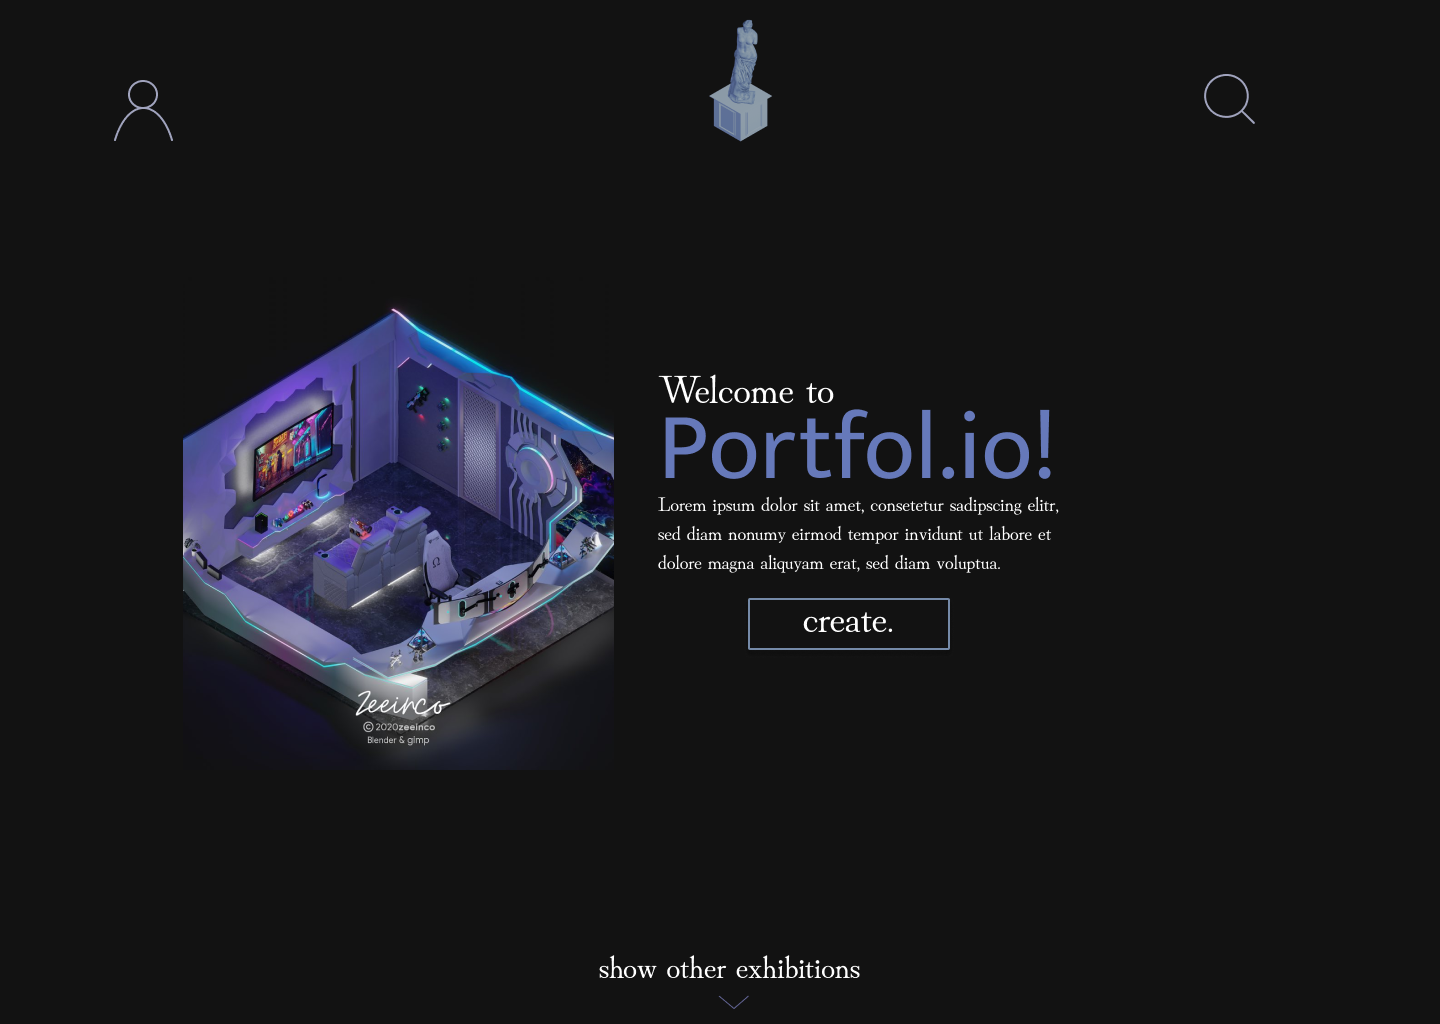
\includegraphics[scale=0.3]{pics/DesignKonzept1_1.png}
    \caption{Design Konzpet 1 Page 1}
\end{figure}

\begin{figure}
    \centering
    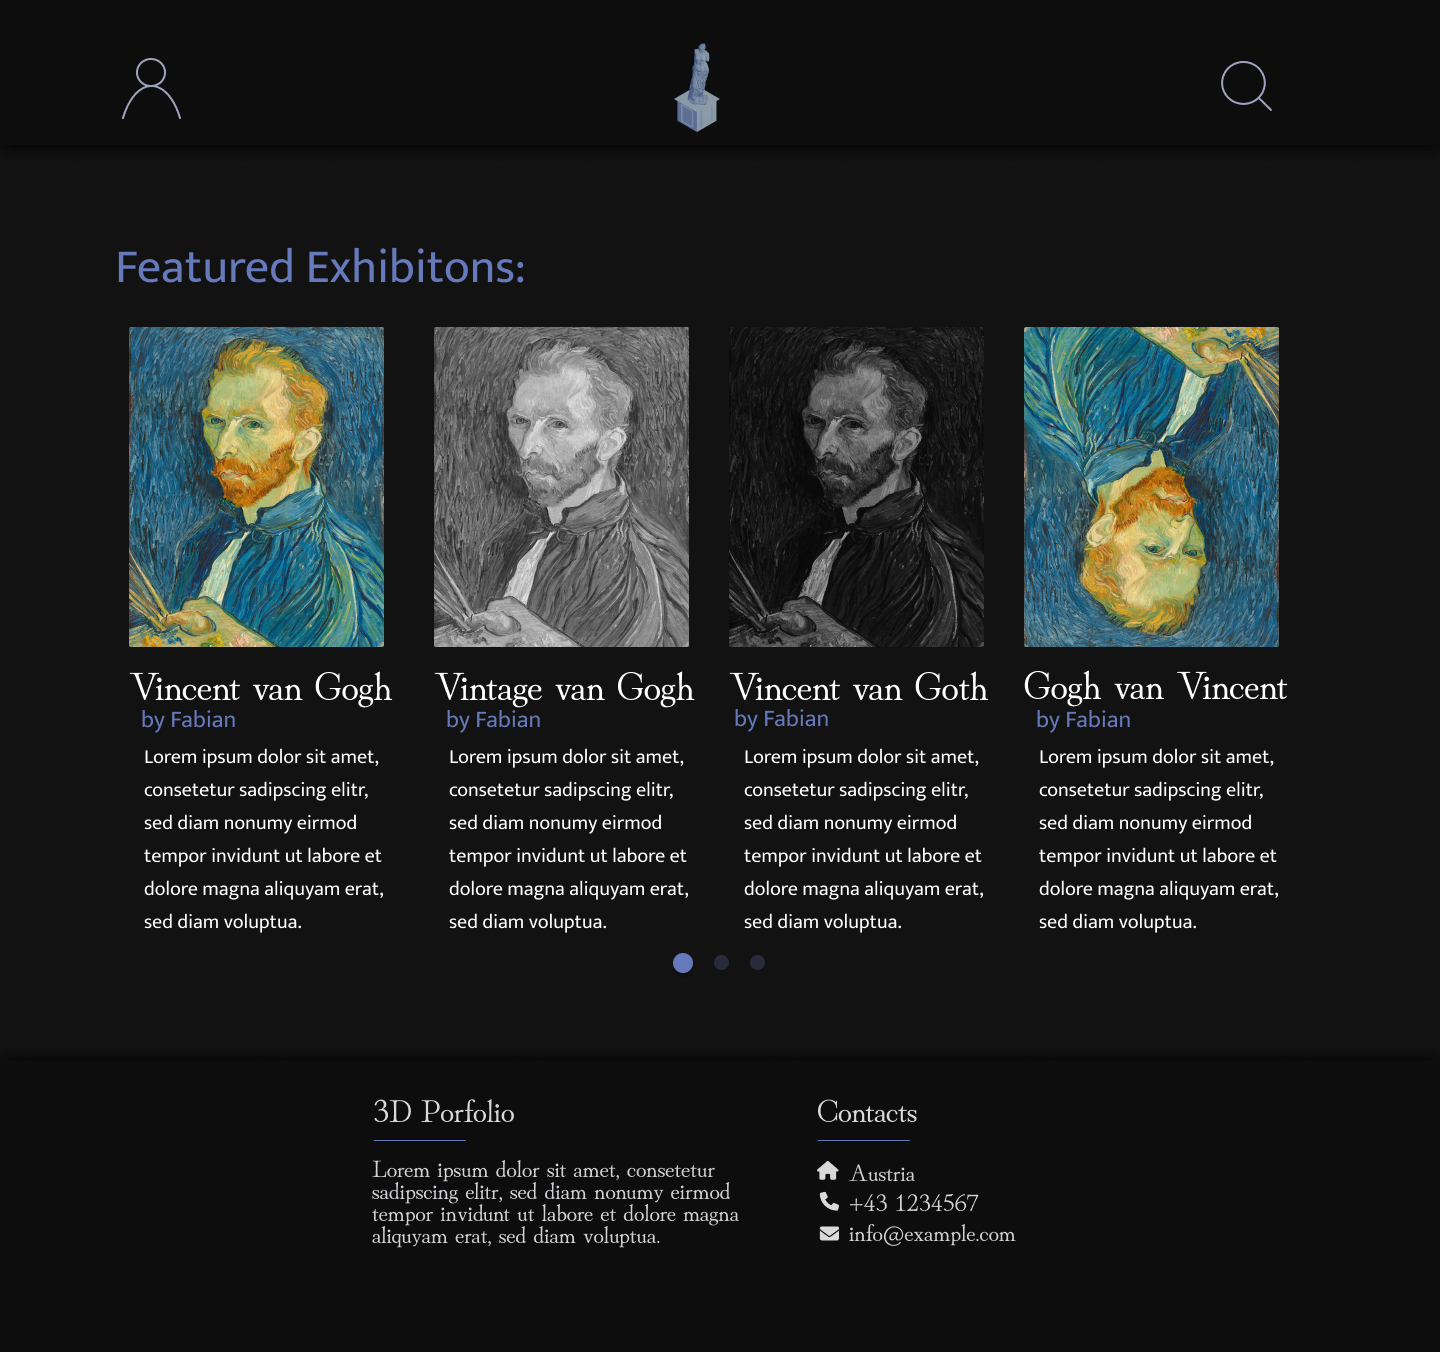
\includegraphics[scale=0.3]{pics/DesignKonzept1_2.png}
    \caption{Design Konzpet 1 Page 2}
\end{figure}

\begin{figure}
    \centering
    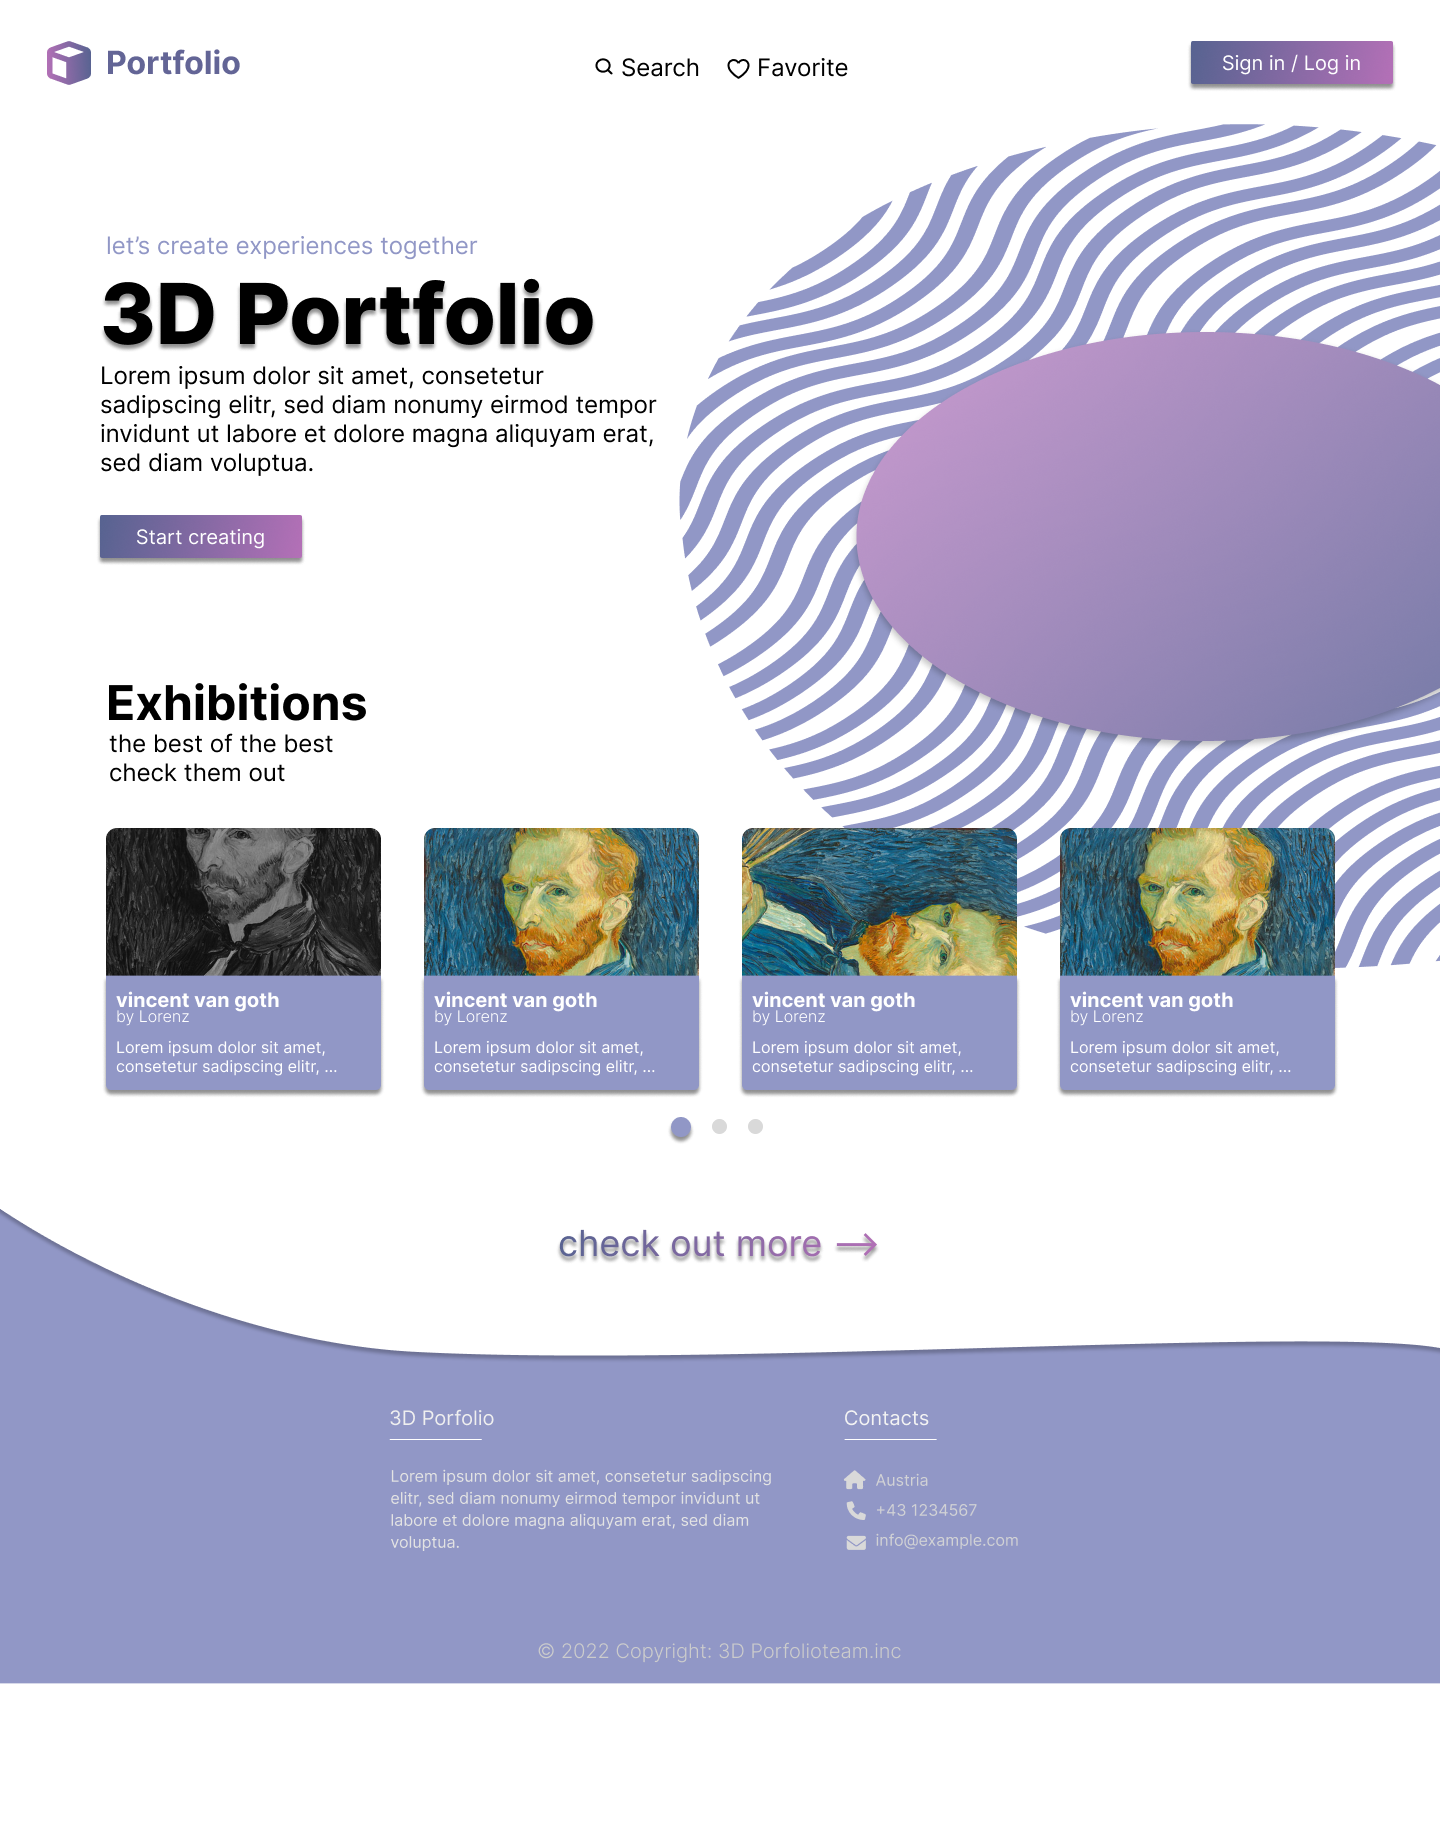
\includegraphics[scale=0.3]{pics/DesignKonzept2.png}
    \caption{Design Konzept 2}
\end{figure}

\subsection{Webseiten Design - Entwicklung [L]}
\setauthor{Litzlbauer Lorenz}
In den vorherigen Kapiteln (Userexperience und Corporate Design) wurde bereits besprochen, wie das Konzept für das Webseiten-Design aussehen sollte und designt wurde. Eine kurze Zusammenfassung: Erst wurde das Corporate Design festgelegt und darauf aufbauend wurden die einzelnen Seiten der Webseite, um die Anforderungen (siehe Seite \pageref{ch:umsetzung:projekt-user-stories} Projekt User Stories) zu erfüllen, designt, dafür wurde das Tool Figma verwendet.

Danach wurde das \emph{Framework} Angular verwendet, um aus den einzelnen Webseiten-Seiten-Angaben eine echte Webseite zu entwickeln. Dabei wurden Userinterface-Frameworks (oder auch Design-Frameworks/Libraries) verwendet, um den Entwicklungsprozess zu beschleunigen.

\subsubsection{UserInterface-Frameworks (UI-Frameworks)}
Ein UserInterface-Frameworks ist eine Ansammlung von Web Komponenten wie eine Navigationsleiste die sofort Nutzbar sind.  


Die Vorteile von UI-Frameworks sind:
\begin{compactitem}
    \item vereinfacht und beschleunigt den Entwicklungsprozess;
    typische Web-Komponenten sind vordefinierte, der Entwickler muss diese nicht mehr implementieren und erspart sich Zeit.
    \item Cross-Browser Unterstützung;
    Besonders bei neuen CSS-Feature kann es sein, dass diese noch nicht von allen Browsern unterstützt werden. Ein UI-Framework benutzt in der Regel nur Funktionen, die auch alle Browser anzeigen können.
    \item Der Code hat eine bessere Lesbarkeit;
    In einem UI-Framework gibt es gewisse Konventionen wie Klassennamen, die befolgt werden müssen. Dadurch wird der Code besser lesbar.
\end{compactitem}


Die Nachteile von UI-Frameworks sind:
\begin{compactitem}
    \item Die Ladezeit der Webseite erhöht sich;
    Schließlich müssen auch mehr Daten an den Browser geschickt werden.
    \item Webseiten, die das selbe UI-Framework verwenden, schauen einander ähnlich aus;
    Da die Web-Komponenten gleich implementiert werden.
\end{compactitem}
\cite{CssFrameworkExplaination} \cite{BestCSSFrameworksin2022}

\subsubsection{UI-Frameworks im Projekt}
Im Projekt wurde sich für zwei UI-Frameworks, Bootstrap und AngularMaterials, entschieden.


\paragraph{Angular Material}
Angular Material ist eine UI Framework und wird seit 2014 von Google entwickelt. Das Framework baut auf Angular auf und erweitert es mit eigenen Komponenten, Styleguides, Typographie und vielem mehr. Die Design-Sprache orientiert sich dabei an der Material Design Spezifikation von Google. Ein großer Fokus des Frameworks ist die Responsiveness, Komponenten werden auf verschiedenen Auflösungen gut aussehen.


Angular Material hat folgende Features:
\begin{compactitem}
    \item Erweiterbar; Bei der Installation lassen sich viele Designanpassungen machen, zusätzlich lassen sich Styles mit dem globalen Stylesheet überschreiben. 
    \item Hochwertig; Die Komponenten sind erprobt und wurden auf die Performanz und Verlässlichkeit getestet.
    \item Reibungslos; Angular Material ist gut mit Angular integriert
\end{compactitem}

Die Abbildung \ref{fig:impl:angular-material-overview-components} zeigt einen Teil der Komponenten, die Angular Material anbietet. Zu allen diesen Komponenten gibt es eine ausführliche Dokumentation mit Beispiele. 
\cite{JavaPointAngularMaterial}
\cite{WhatAngularMaterial}

\begin{figure}
    \centering
    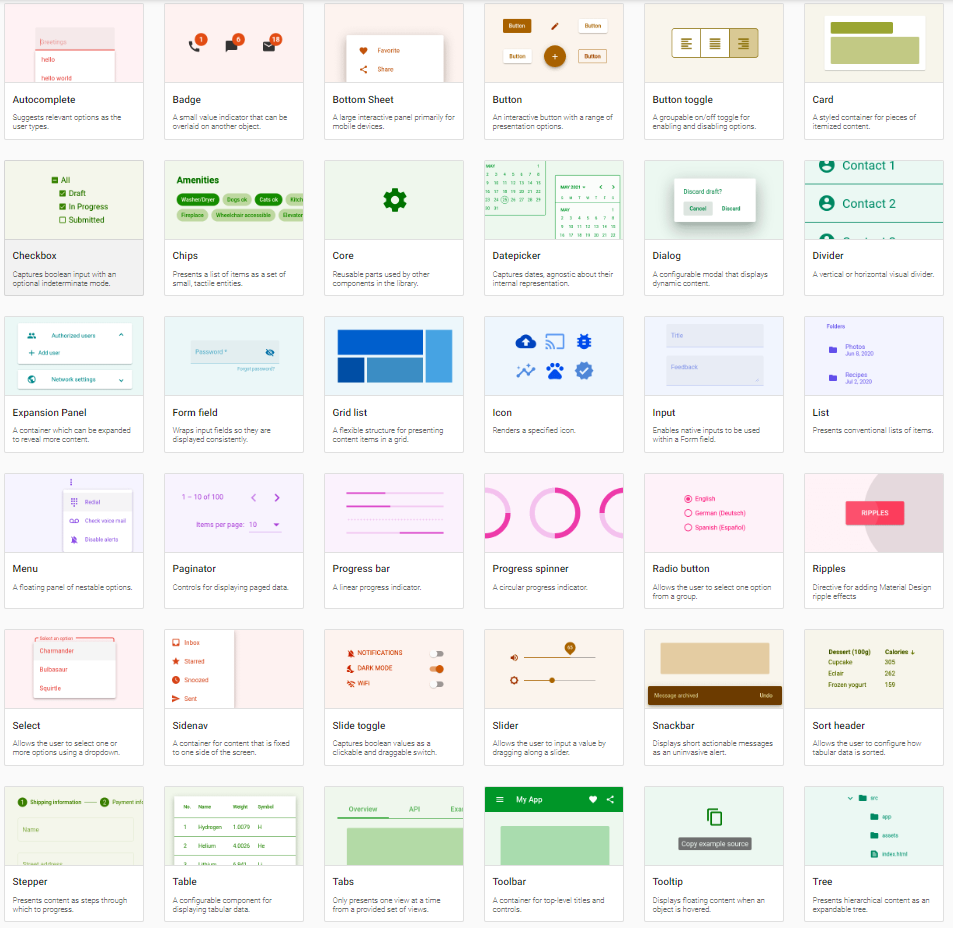
\includegraphics[scale=0.5]{pics/AngularMaterialsComponentsOverview.png}
    \caption{Angular Material: Komponente Überblick}
    \label{fig:impl:angular-material-overview-components}
\end{figure}
Abbildung \ref{fig:impl:angular-material-overview-components} \cite{AngularComponents}

\subparagraph{Material Design Spezifikation}
Material Design ist ein Designsystem, welches von Google erstellt wurde, um Teams zu helfen, qualitative hochwertige Digitale-Erfahrungen für Android, iOS, Flutter und das Web zu gestalten.

Material Design hat mehrere Prinzipien, die sie ihr Design beeinflussen lassen.

Material Design soll die reale Weld abbilden.
Text soll durch Typographie, Raster, Abstände, Farben und Bilder soll eine erkennbare Hierarchie entstehen. Komponenten sind interaktive Bauklötze für ein das User Interface. Komponenten haben alle eine Stati-System welches den Status der Komponente fokussiert, selektiert, aktiviert, fehlerhaft, schwebend, gedrückt und ausgeschalten anzeigt. Durch das Theming ist es möglich einzelne Komponenten zu verändern und das Design so anzupassen, dass es zur Corporate Identity der Benutzer*in passt.
Material Design befasst sich mit den Design-Fundamenten:
\begin{compactitem}
    \item Umgebung
    \item Layout
    \item Navigation
    \item Farbe
    \item Typographie
    \item Ton
    \item Ikonografie
    \item Form
    \item Bewegung
    \item Interaktion
    \item Kommunikation
    \item maschinelles Lernen
\end{compactitem}
\cite{MaterialDesign-Introduction}

\paragraph{Bootstrap}
Bootstrap ist ein kostenloses Open-Source-UI-Framework. Es ist nicht nur eine Ansammlung von CSS sondern auch von JavaScript und HTML code um schöne, interaktive und responsive Webseiten. 

Bootstrap hat folgenden Features: 
\begin{compactitem}
    \item Web-Komponenten, die sofort Anwendbar sind
    \item Eine gute Dokumentation
    \item Mobile Centered Design
    \item Hohe Benutzerfreundlichkeit
\end{compactitem}
\cite{BestCSSFrameworksin2022}

\subsubsection{Scss}
SCSS ist kein UI-Framework, sondern vielmehr eine Syntax- und Feature-Erweiterung von CSS, deswegen wurde es schlussendlich auch für dieses Projekt gewählt. SCSS hat viele Vorteile wie zum Beispiel Variablen, Schleifen, Mixins und Imports gegenüber CSS, aber besonders ausschlaggebend war das Prinzip der Verschachtelung.

Durch die Verschachtelung kann an redundanten Styles-Selektoren gespart werden, was die Style-Definition besser lesbarer macht. Im den Beispielen (siehe SCSS-Code-Beispiel \ref{lst:imp:design:scss} und natives CSS-Code-Beispiel \ref{lst:imp:design:css}) wird die gleiche Style-Definition von SCSS und CSS ausgedrückt, doch die Schreibweise unterscheidet sich.

\cite[Sass Guide]{SassGuide}

\begin{lstlisting}[caption=SCSS - Code Beispiel,label=lst:imp:design:scss]
nav {
    ul {
        margin: 0;
        padding: 0;
        list-style: none;
    }
    
    li { display: inline-block; }
    
    a {
        display: block;
        padding: 6px 12px;
        text-decoration: none;
    }
}
\end{lstlisting}

\begin{lstlisting}[caption=CSS - Code Beispiel,label=lst:imp:design:css]
nav ul {
    margin: 0;
    padding: 0;
    list-style: none;
    }
nav li {
    display: inline-block;
    }
nav a {
    display: block;
    padding: 6px 12px;
    text-decoration: none;
}
\end{lstlisting}

Code Beispiele\ref{lst:imp:design:scss} \ref{lst:imp:design:css} \cite[Sass Guide]{SassGuide}




